\usetikzlibrary{calc}
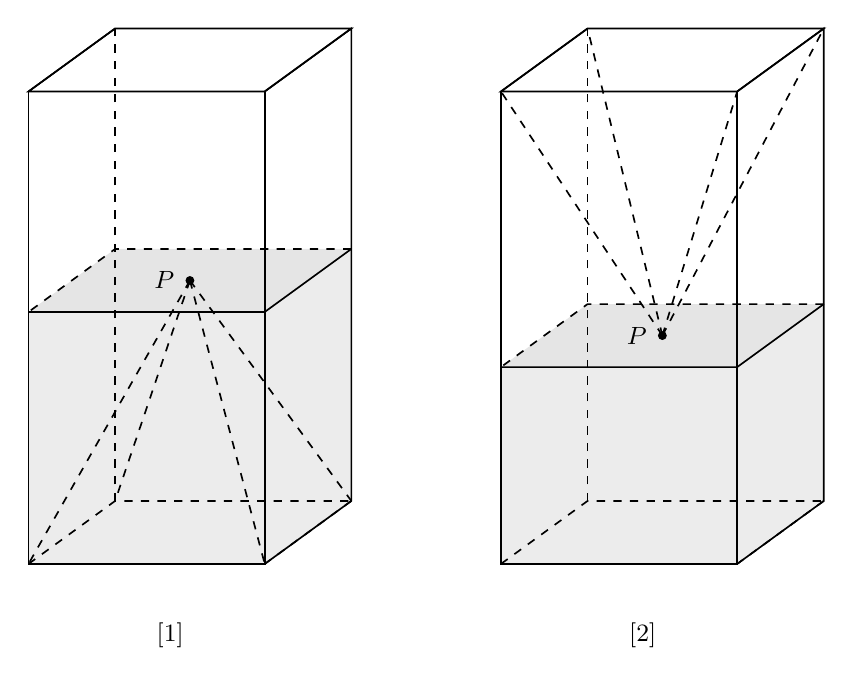
\begin{tikzpicture}[line width=.6pt, >=stealth, font=\small]
% ---- left panel (Fig.1) ----
\coordinate (LFLB) at (0,0);
\coordinate (LFRB) at (3,0);
\coordinate (LFLT) at (0,3.2);
\coordinate (LFRT) at (3,3.2);
\coordinate (LFLTu) at (0,6);
\coordinate (LFRTu) at (3,6);
\coordinate (LBLB) at (1.1,0.8);
\coordinate (LBRB) at (4.1,0.8);
\coordinate (LBLT) at (1.1,4.0);
\coordinate (LBRT) at (4.1,4.0);
\coordinate (LBLTu) at (1.1,6.8);
\coordinate (LBRTu) at (4.1,6.8);
\coordinate (LP) at (2.05,3.6);
% water shading (lower volume + surface)
\fill[gray!15] (LFLB)--(LFRB)--(LFRT)--(LFLT)--cycle;
\fill[gray!15] (LFRB)--(LBRB)--(LBRT)--(LFRT)--cycle;
\fill[gray!20] (LFLT)--(LFRT)--(LBRT)--(LBLT)--cycle;
% solid outer box
\draw (LFLB)--(LFRB)--(LFRTu)--(LFLTu)--cycle;
\draw (LFRB)--(LBRB)--(LBRTu)--(LFRTu);
\draw (LFLTu)--(LFRTu)--(LBRTu)--(LBLTu)--cycle;
\draw (LFLTu)--(LBLTu);
% water plane
\draw (LFLT)--(LFRT)--(LBRT);
\draw[dashed] (LBRT)--(LBLT)--(LFLT);
% bottom hidden
\draw[dashed] (LFLB)--(LBLB)--(LBRB);
\draw[dashed] (LBRB)--(LFRB);
% back-left vertical hidden
\draw[dashed] (LBLB)--(LBLTu);
% pyramid P to bottom corners
\draw[dashed] (LP)--(LFLB);
\draw[dashed] (LP)--(LFRB);
\draw[dashed] (LP)--(LBRB);
\draw[dashed] (LP)--(LBLB);
\fill (LP) circle (1.6pt);
\node[left=2pt] at (LP) {$P$};
\node at (1.8,-0.9) {\bitmapinsertcaption[1]};
% ---- right panel (Fig.2) ----
\coordinate (RFLB) at (6,0);
\coordinate (RFRB) at (9,0);
\coordinate (RFLT) at (6,2.5);
\coordinate (RFRT) at (9,2.5);
\coordinate (RFLTu) at (6,6);
\coordinate (RFRTu) at (9,6);
\coordinate (RBLB) at (7.1,0.8);
\coordinate (RBRB) at (10.1,0.8);
\coordinate (RBLT) at (7.1,3.3);
\coordinate (RBRT) at (10.1,3.3);
\coordinate (RBLTu) at (7.1,6.8);
\coordinate (RBRTu) at (10.1,6.8);
\coordinate (RP) at (8.05,2.9);
\fill[gray!15] (RFLB)--(RFRB)--(RFRT)--(RFLT)--cycle;
\fill[gray!15] (RFRB)--(RBRB)--(RBRT)--(RFRT)--cycle;
\fill[gray!20] (RFLT)--(RFRT)--(RBRT)--(RBLT)--cycle;
\draw (RFLB)--(RFRB)--(RFRTu)--(RFLTu)--cycle;
\draw (RFRB)--(RBRB)--(RBRTu)--(RFRTu);
\draw (RFLTu)--(RFRTu)--(RBRTu)--(RBLTu)--cycle;
\draw (RFLTu)--(RBLTu);
\draw (RFLT)--(RFRT)--(RBRT);
\draw[dashed] (RBRT)--(RBLT)--(RFLT);
\draw[dashed] (RFLB)--(RBLB)--(RBRB);
\draw[dashed] (RBRB)--(RFRB);
\draw[dashed] (RBLB)--(RBLTu);
\draw[dashed] (RP)--(RFLTu);
\draw[dashed] (RP)--(RFRTu);
\draw[dashed] (RP)--(RBRTu);
\draw[dashed] (RP)--(RBLTu);
\fill (RP) circle (1.6pt);
\node[left=2pt] at (RP) {$P$};
\node at (7.8,-0.9) {\bitmapinsertcaption[2]};
\end{tikzpicture}
